\documentclass[12pt]{article}
\usepackage[UTF8]{ctex}
\usepackage{geometry}
\usepackage{listings}
\usepackage{graphicx}
\usepackage{subfigure}
\usepackage{array}
\usepackage{caption}    
\usepackage{float}
\usepackage{subfloat}
\usepackage{hyperref}
\usepackage{bookmark}
\usepackage{amsmath}
\usepackage{url}
\usepackage{amsfonts,amssymb}

\geometry{left=15mm,right=15mm,top=20mm,bottom=20mm}
\title{第十次作业报告}
\author{PB21010362 汪兆辰}
\date{\today}
\newcommand{\upcite}[1]{\textsuperscript{\textsuperscript{\cite{#1}}}}

\begin{document}

\maketitle

\section{算法介绍}
在得到正交投影之前,需要先对给定的物体进行变形,将需要渲染的物体映射到x,y,z轴的[-1,1]范围内.为了定义正交投影变换,需要先将相机坐标固定在世界坐标中,定义长方体视锥体,并将视锥体移动到相机坐标的中心并归一化.由于在OpenGL中z轴的正方向指向屏幕外,但视觉上我们认为
距离越远的地方z坐标应该越大,所以需要将z轴反向变为左手系.

首先定义平移矩阵:
\begin{equation}
    M_T=
    \begin{pmatrix}
        1&0&0&-\frac{left+right}{2}\\
        0&1&0&-\frac{top+bottom}{2}\\
        0&0&1&-\frac{zFar+zNear}{2}\\
        0&0&0&1
    \end{pmatrix}
\end{equation}

再定义缩放矩阵:
\begin{equation}
    M_S=
    \begin{pmatrix}
        \frac{2}{right-left}&0&0&0\\
        0&\frac{top-bottom}{2}&0&0\\
        0&0&\frac{zFar-zNear}{2}&0\\
        0&0&0&1\\
    \end{pmatrix}
\end{equation}

从而得到:
\begin{equation}
    M_{Ortho}=M_{-z}M_S M_T
\end{equation}

即:
\begin{equation}
    M_{Ortho}=\begin{pmatrix}
        \frac{2}{right-left}&0&0&-\frac{left+right}{2}\\
        0&\frac{2}{top-bottom}&0&-\frac{top+bottom}{2}\\
        0&0&\frac{-2}{zFar-zNear}&-\frac{zFar+zNear}{2}\\
        0&0&0&1
    \end{pmatrix}
\end{equation}
其中$M_{-z}$使得z轴反向.

在代码中只需要将原来的透视投影所用的矩阵变为(4)式中的矩阵即可,注意到视锥的宽与高需要满足比例为aspect,在给定参数时只需要给定宽与aspect即可,代码实现如下:
\begin{lstlisting}
Eigen::Matrix4f orthographic(float left,float right,float aspect,
 float zNear, float zFar) const{
    assert(zFar > zNear);
    float top = left / aspect;
    float bottom = right / aspect;
    Eigen::Matrix4f res = Eigen::Matrix4f::Zero();
    res(0, 0) = 2 / (right - left);
    res(1, 1) = 2 / (top - bottom);
    res(2, 2) = 2 / (zNear - zFar);
    res(3, 3) = 1;
    res(0, 3) = -(right + left) / 2;
    res(1, 3) = -(bottom + top) / 2;
    res(2, 3) = -(zFar + zNear) / 2;
    return res;
}
    
\end{lstlisting}

\section{效果展示}

\begin{figure}[htbp]
    \centering
    \subfigure[Orthographic]{
        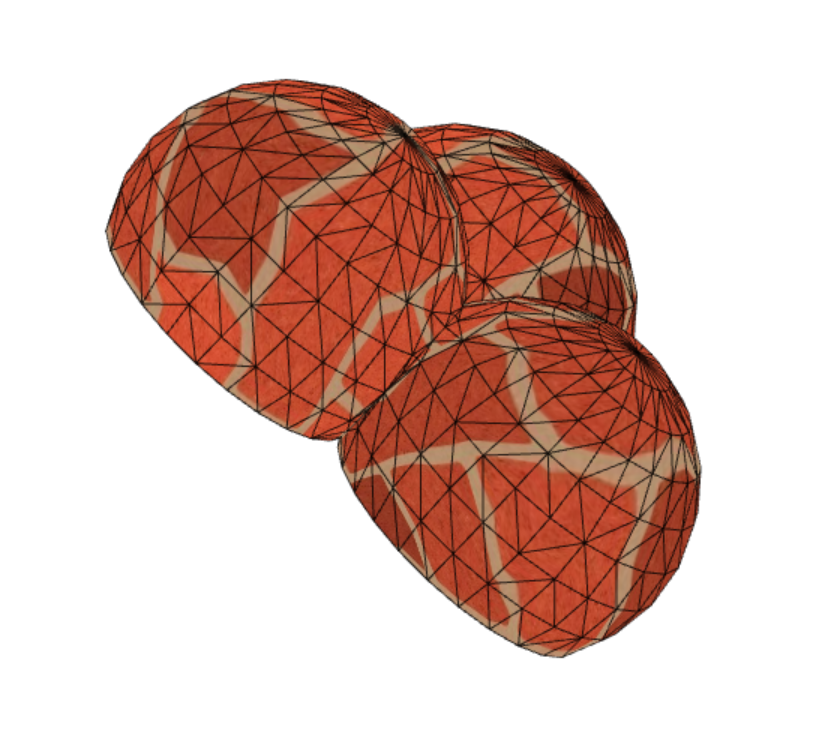
\includegraphics[width=0.25\textwidth]{pic01.png}
    }
    \subfigure[Perspective]{
        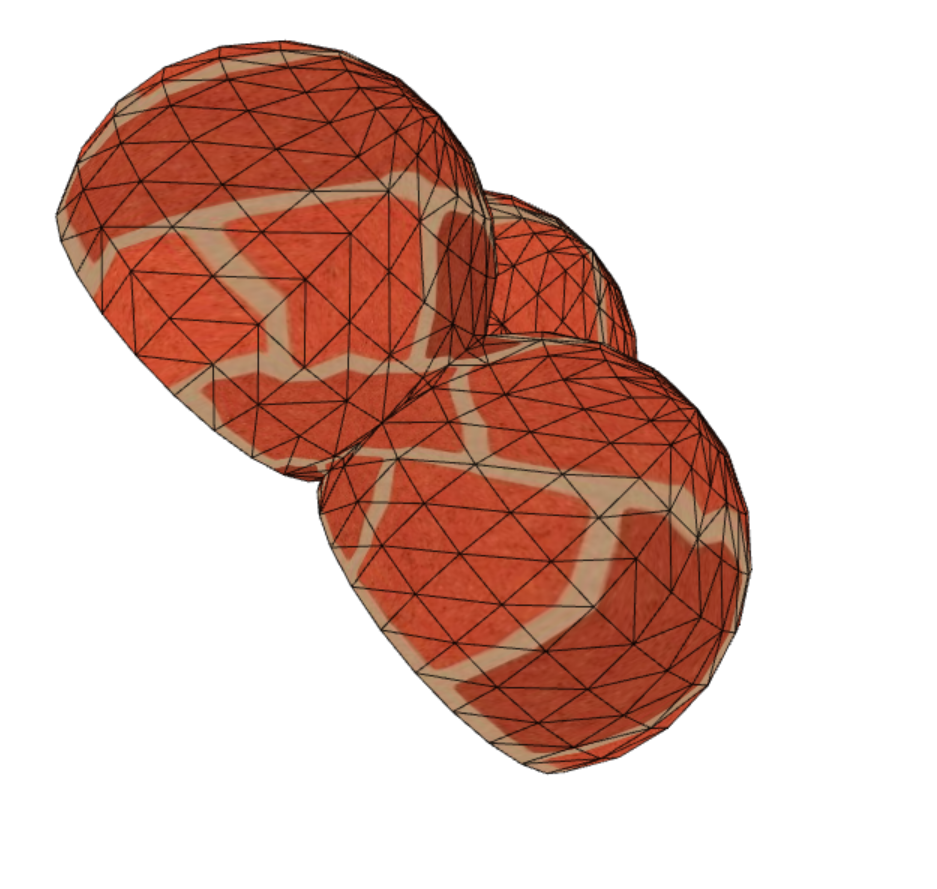
\includegraphics[width=0.25\textwidth]{pic02.png}
    }
\end{figure}

可以看到,正交投影不考虑物体的远近,在相同角度下远处的半球明显大于透视投影.

\section{计算参数}
如果只使用透视投影的参数也可以计算出需要的六个参数. 其中fovy为相机坐标到视锥上下的张角,aspect为宽高比,zFar与zNear对应
到视锥的前后距离. 不妨设视锥关于x,y轴对称,即
\begin{equation}
    top+bottom=left+right=0
\end{equation}
由参数的几何意义容易得出$top=zNear \cdot \tan\frac{fovy}{2}$,$right=top\cdot aspect$.

由此生成的投影图像如下:
\begin{figure}[htbp]
    \centering
    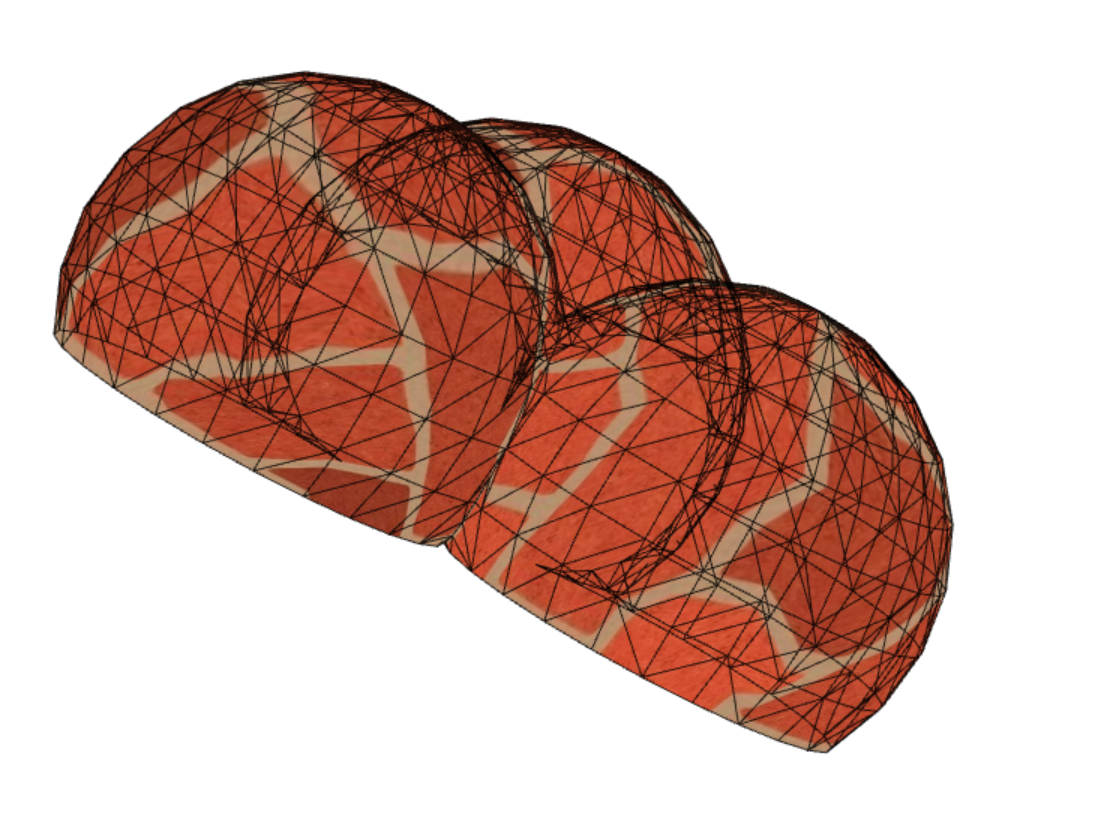
\includegraphics[scale=0.5]{pic03.png}
\end{figure}
这时模型变“透明”了,可能是z-buffer精度丢失导致,而且最初生成的图像过大,需要手动缩小,于是考虑处理top的计算参数.

如果令$top=zFar\cdot  \tan\frac{fovy}{2}$,这时最初生成的图像很小,需要手动放大,并且视锥的前后偏小,导致部分模型被前后截面裁掉.
\begin{figure}[htbp]
    \centering
    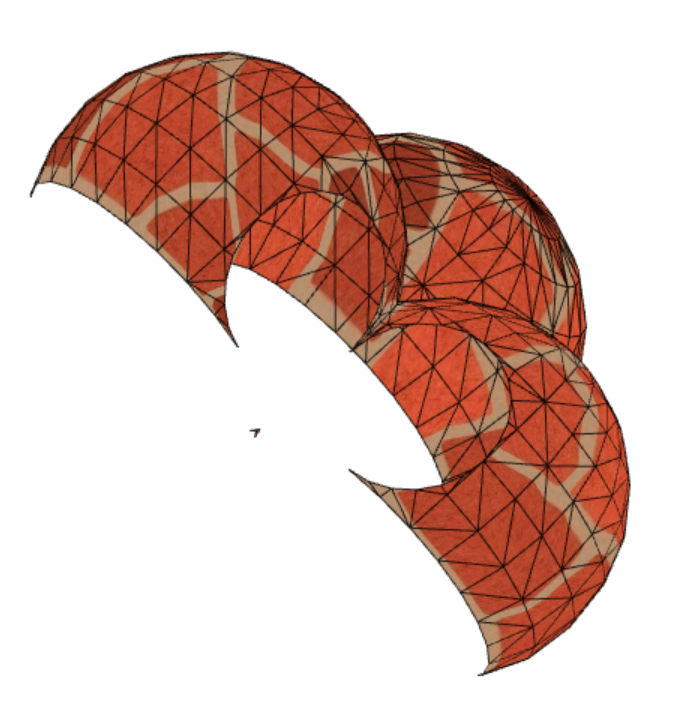
\includegraphics[scale=0.5]{pic04.png}
\end{figure}

于是希望可以在zFar与zNear之间寻找到一个较合适的参数,经过调试发现当$$top=0.04\cdot zFar\cdot \tan\frac{fovy}{2}$$时能得到较为理想的效果.

\newpage

\begin{figure}[htbp]
    \centering
    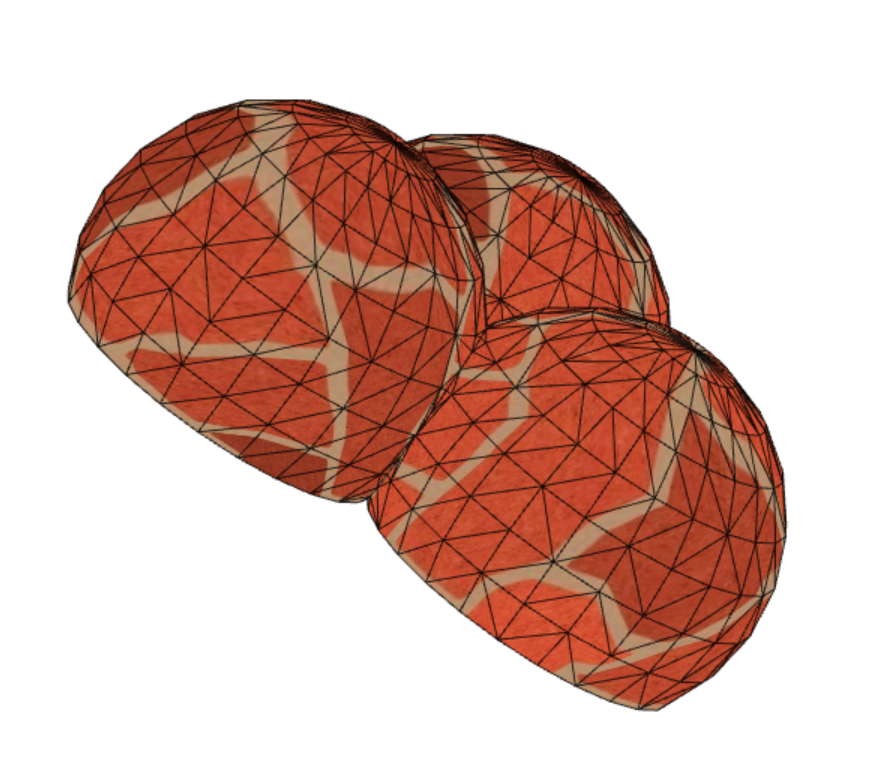
\includegraphics[scale=0.5]{pic05.png}
\end{figure}


\begin{thebibliography}{3}
    \bibitem{1} \url{https://www.bilibili.com/video/BV12t4y1c7zd/}
    \bibitem{2} \url{https://blog.csdn.net/u011418943/article/details/128052420}
\end{thebibliography}


\end{document}